

\documentclass{article}
\usepackage{amsmath, amssymb, graphicx, subcaption}  % For \mathbb command


    \title{Practicas MC}
    \date{\today}
    \author{Juan Luis Torres Ramos}

    \begin{document}
        
        % 
        % Portada
        % \pagenumbering{gobble}
        % \maketitle
        % \newpage
        % \pagenumbering{arabic}

        \begin{titlepage}
            \centering
            {
\includegraphics[width=1\textwidth]{./Imagenes/logo_universidad_de_granada.png}\par}
            \vspace{1cm}
            {\scshape\Large Escuela Tecnica Superior de Ingenieria Informatica y Telecomunicaciones \par}
            \vspace{2.5cm}
            {\scshape\Huge Practicas Modelos de Computación \par}
            \vspace{1cm}
            {\itshape\Large  Grupo B3 \par} 
            \vfill
            {\Large Juan Luis Torres Ramos \par}
            {\Large 24 Octubre 2023 \par}
            \end{titlepage}


        % introducción
        \section*{Practica 1}
        Encuentra una gramática libre del contexto para generar cada uno de los siguientes lenguajes:

        \begin{enumerate}
            \item $L = \{a^i b^j \, | \, i, j \in \mathbb{N}, \, i \leq j\}$.
            \item $L = \{a^i b^j a^j b^i \, | \, i, j \in \mathbb{N}\}$.
            \item $L = \{a^i b^i a^j b^j \, | \, i, j \in \mathbb{N}\}$.
            \item $L = \{a_i b_i \,|\, i \in \mathbb{N}\} \cup \{b_i a_i \,|\, i \in \mathbb{N\}}$.
            \item $L = \{uu^{-1} \mid u \in \{a, b\}^*\}$.
            \item $L = \{a^i b^j c^{i+j} \, | \, i, j \in \mathbb{N}\}$.    
        \end{enumerate}

        \begin{flushleft}
            donde $\mathbb{N}$ es el conjunto de los numeros naturales incluyendo el 0
        \end{flushleft}


        \vspace{\baselineskip} % paso linea


        % Pasos que voy a seguir para resolver el ejercicio
        \begin{flushleft}
            
            \subsubsection*{Pasos para resolver el ejercicio:}
                        
            \begin{enumerate}
                \item Determinar los símbolos terminales y no terminales.
                \item Determinar el símbolo inicial.
                \item Analizar el lenguaje para determinar qué se pide.
                \item Determinar las reglas de producción.
                \item Comprobar con JFLAP  
            \end{enumerate}
        \end{flushleft}


        \newpage

        % 
        % APARTADO 1

        \subsection*{A. $L = \{a^i b^j \, | \, i, j \in \mathbb{N}, \, i \leq j\}$.}

        \begin{flushleft}
            \begin{enumerate}
                \item Los símbolos terminales serán $\{a,b\}$ y los simbolos no terminales serán $S$ y $B$.
                \item El símbolo inicial será $S$.
                \item Analizar el lenguaje para determinar qué se pide. En este caso, se pide que la cadena tenga un número de $a$ menor o igual que el número de $b$. Por ejemplo, $aabbb$ y $aabb$ pertenecen al lenguaje, pero $aab$ no.
                \item Determino las reglas de producción:
                \begin{itemize}
                    \item $S \rightarrow \epsilon$ (genero la cadena vacía).
                    \item $S \rightarrow aSb$.
                    \item $S \rightarrow Sb$.
                \end{itemize}

                \item compruebo con JFLAP que la gramática es correcta.
                
                \vspace{\baselineskip} % paso linea

                % Imagenes en matriz
                \begin{figure}[h] 
                    \centering
                    \begin{subfigure}[b]{0.45\textwidth}
                        \centering
                        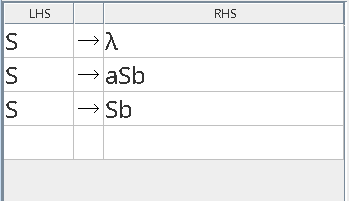
\includegraphics[width=\textwidth]{./Imagenes/produccion1.png}
                        \caption{la producción}
                        \label{fig:label1}
                    \end{subfigure}
                    \hfill
                    \begin{subfigure}[b]{0.45\textwidth}
                        \centering
                        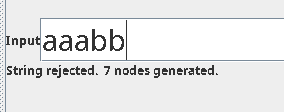
\includegraphics[width=\textwidth]{./Imagenes/grafoaaabb.png}
                        \caption{la cadena $aaabb$}
                        \label{fig:label2}
                    \end{subfigure}
                    \vspace{0.5cm} 
                    \\
                    \begin{subfigure}[b]{0.45\textwidth}
                        \centering
                        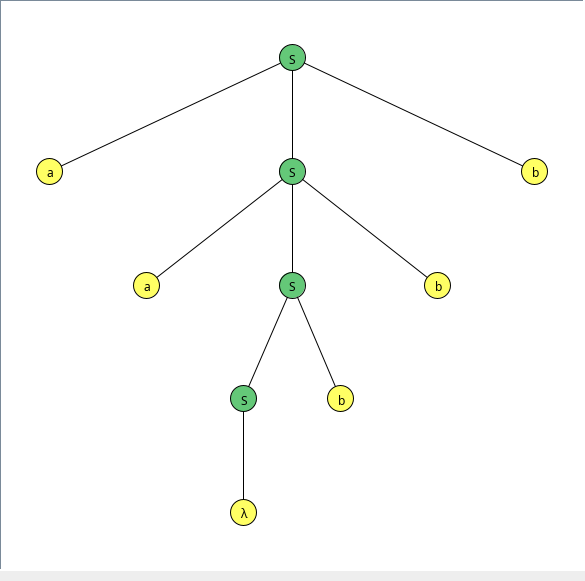
\includegraphics[width=\textwidth]{./Imagenes/grafoaabbb.png}
                        \caption{la cadena $aabbb$}
                        \label{fig:label3}
                    \end{subfigure}
                    \hfill
                    \begin{subfigure}[b]{0.45\textwidth}
                        \centering
                        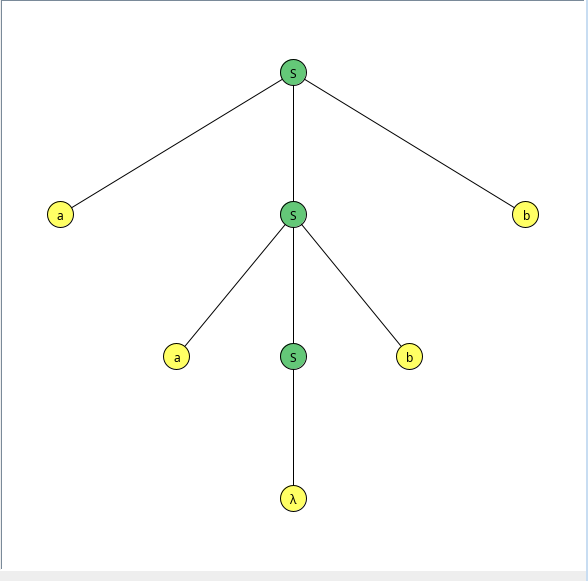
\includegraphics[width=\textwidth]{./Imagenes/grafoaabb.png}
                        \caption{la cadena $aabb$}
                        \label{fig:label4}
                    \end{subfigure}
                    \label{fig:matrix1}
                \end{figure}

                

                 

            \end{enumerate}
        \end{flushleft}

        % 
        % Apartado 2

        \newpage % paso pagina
        \subsection*{B. $L = \{a^i b^j a^j b^i \, | \, i, j \in \mathbb{N}\}$.}
        \begin{flushleft}
            \begin{enumerate}

                \item Los símbolos terminales serán $\{a,b\}$ y los simbolos no terminales serán $S$ y $B$.

                \item El símbolo inicial será $S$.
            
                \item El lenguaje nos pide generar una cadena de 4 caracteres donde primero se generen $a^i b^j$ y luego $a^j b^i$, es decir en los extremos un numero caracteres $i$ y en los caracteres del centro un numero de caracteres $j$. 
                Por ejemplo, $aababb$ y $ab$ pertenecen al lenguaje, pero $aabbab$ no.

                \item Determino las reglas de producción:
                \begin{itemize}
                    \item $S \rightarrow aSb$ (genero mismo numero de caracteres en los extremos).
                    \item $S \rightarrow B$.
                    \item $B \rightarrow bBa$ (genero mismo numero de caracteres en el centro).
                    \item $B \rightarrow \epsilon$ (genero la cadena vacía).
                \end{itemize}

                \item compruebo con JFLAP que la gramática es correcta.

                % Imagenes en matriz
                \begin{figure}[h] 
                    \centering
                    \begin{subfigure}[b]{0.4\textwidth}
                        \centering
                        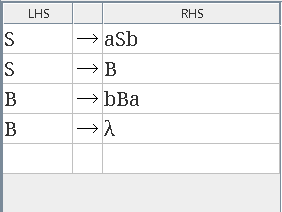
\includegraphics[width=\textwidth]{./Imagenes/produccion2.png}
                        \caption{la producción}
                        \label{fig:label5}
                    \end{subfigure}
                    \hfill
                    \begin{subfigure}[b]{0.4\textwidth}
                        \centering
                        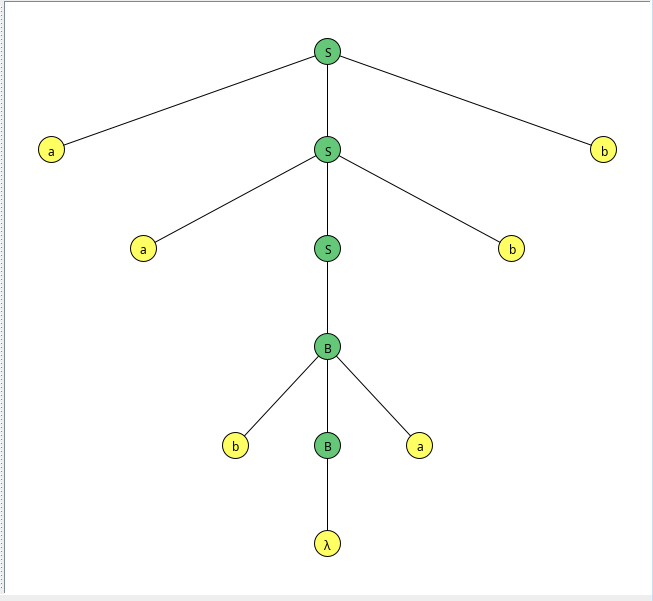
\includegraphics[width=\textwidth]{./Imagenes/grafo1.png}
                        \caption{la cadena $aababb$}
                        \label{fig:label6}
                    \end{subfigure}
                    \vspace{0.5cm} 
                    \\
                    \begin{subfigure}[b]{0.4\textwidth}
                        \centering
                        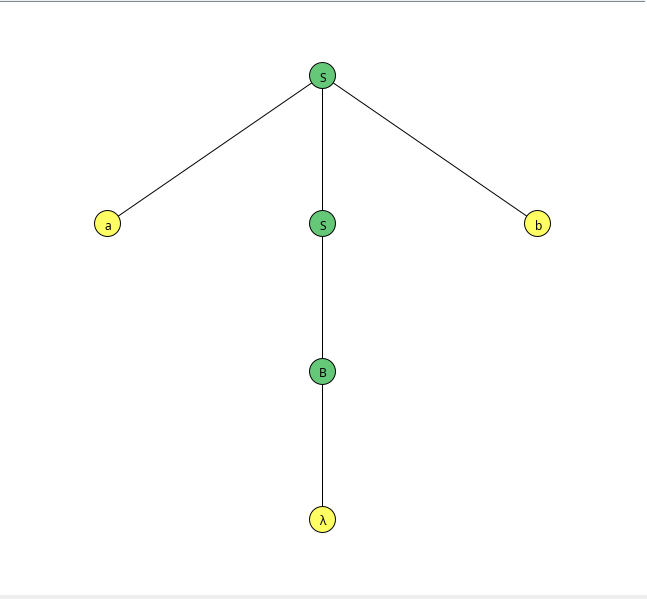
\includegraphics[width=\textwidth]{./Imagenes/grafo2.png}
                        \caption{la cadena $ab$}
                        \label{fig:label7}
                    \end{subfigure}
                    \hfill
                    \begin{subfigure}[b]{0.4\textwidth}
                        \centering
                        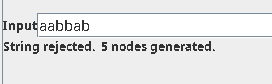
\includegraphics[width=\textwidth]{./Imagenes/grafo3.png}
                        \caption{la cadena $aabbab$}
                        \label{fig:label8}
                    \end{subfigure}
                    \label{fig:matrix2}
                \end{figure}

            \end{enumerate}
        \end{flushleft}
        
        
        % 
        % Apartado 3



    \end{document}
